

\def\expansion{
%
\begin{align*}
%
\expect{p(\theta \vert \xvec, \w)}{f(\theta)} -
    \expect{p(\theta \vert \xvec)}{f(\theta)} ={}&
    \sumn \blue{\infl_n} (\w_n - 1) + \red{\err(\w)}
%
\end{align*}
%
}





%%%%%%%%%%%%%%%%%%%%%%%%%%%%%%%%%%%%%%%%%%%%%%%%%%%%%%%%%%%%%%
%%%%%%%%%%%%%%%%%%%%%%%%%%%%%%%%%%%%%%%%%%%%%%%%%%%%%%%%%%%%%%
%%%%%%%%%%%%%%%%%%%%%%%%%%%%%%%%%%%%%%%%%%%%%%%%%%%%%%%%%%%%%%


\begin{frame}{Data re-weighting.}


\onslide<1->{
Augment the problem with {\em data weights} $\w_1, \ldots, \w_N$.
}
\onslide<2->{
%
\begin{align*}
%
\ell_n(\theta) :={}& \log \p(\x_n \vert \theta)
&
\log \p(\xvec \vert \theta, \w) ={}&
    \sumn \w_n \ell_n(\theta)
&
\Rightarrow \text{We write }\expect{\p(\theta \vert \xvec, \w)}{f(\theta)}.
    %
\end{align*}
}

\begin{minipage}{0.49\textwidth}
    \onslide<2-> {
    Original weights: \par
    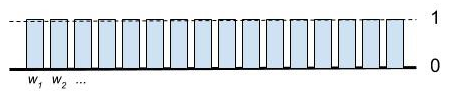
\includegraphics[width=0.78\textwidth]{static_figures/orig_weights}
    }
    \onslide<3-> {
    \par Leave-one-out weights: \par
    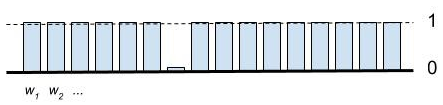
\includegraphics[width=0.78\textwidth]{static_figures/weights_loo}
    }
    \onslide<4-> {
    \par Bootstrap weights: \par
    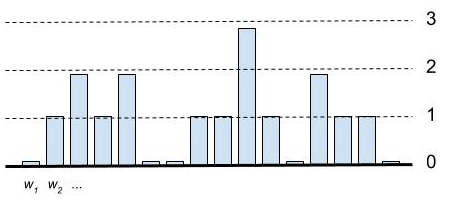
\includegraphics[width=0.78\textwidth]{static_figures/boot_weights}
    }
\end{minipage}
%\onslide<1->{
\begin{minipage}{0.49\textwidth}
    % https://www.overleaf.com/learn/latex/TikZ_package
    % https://latexdraw.com/how-to-annotate-an-image-in-latex/
    % https://tex.stackexchange.com/questions/9559/drawing-on-an-image-with-tikz
    \begin{tikzpicture}
        \onslide<5-> {
        \node[anchor=south west,inner sep=0] (image) at (0,0) {
            %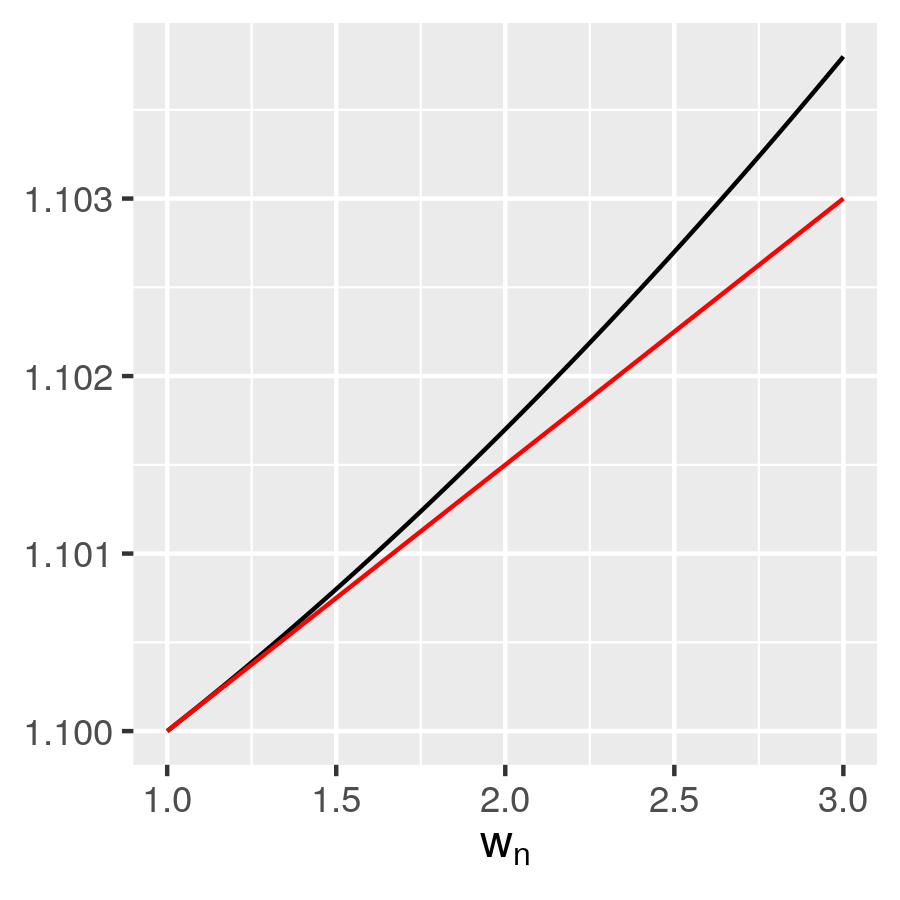
\includegraphics[width=0.98\textwidth]{static_figures/weight_slope}
            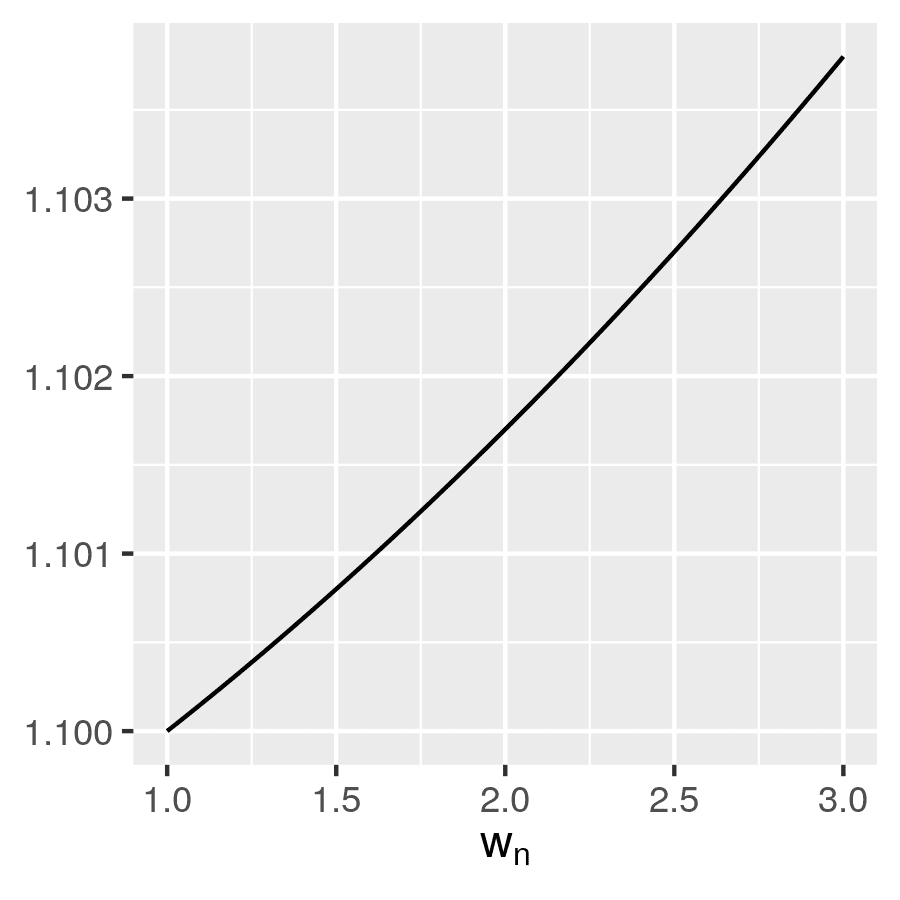
\includegraphics[width=0.98\textwidth]{static_figures/e_beta_w}
        };
        }
        \onslide<7->{
        \begin{scope}[x={(image.south east)},y={(image.north west)}]
            \draw[gray, thick, <-] (0.20,0.23) -- ++(0.15,0.3)
                    node[above,black,fill=white]
                    {\small $\expect{p(\theta \vert \x)}{f(\theta)}$};
        \end{scope}
        }
        \onslide<6->{
        \begin{scope}[x={(image.south east)},y={(image.north west)}]
            \draw[gray, thick, <-] (0.8,0.8) -- ++(-0.1,0.1)
                    node[left,black,fill=white]
                    {\small $\expect{p(\theta \vert \x, \w_n)}{f(\theta)}$};
        \end{scope}
        }
        \onslide<8->{
        \begin{scope}[x={(image.south east)},y={(image.north west)}]
            \draw[blue, thick, -] (0.18,0.18) -- ++(1.2 * 0.6, 1.2 * 0.48);
        \end{scope}
        }
        \onslide<9->{
        \begin{scope}[x={(image.south east)},y={(image.north west)}]
            \draw[gray, thick, <-] (0.4,0.35) -- ++(0.2,-0.08)
                    node[right,black,fill=white]
                    {\small Slope $ = \blue{\infl_n}$};
        \end{scope}
        }
        \onslide<10->{
        \begin{scope}[x={(image.south east)},y={(image.north west)}]
            \draw[gray, thick, <-] (0.8,0.65) -- ++(0.02,-0.2)
                    node[below,black,fill=white]
                    {\small Error $ = \red{\err(\w)}$};
            \draw[red, to-to] (0.8,0.76) -- ++(0,-0.07);
        \end{scope}
        }
    \end{tikzpicture}
%}
\end{minipage}

\onslide<11->{
The re-scaled slope $N \infl_n$ is known as the
``influence function'' at data point $\x_n$.
%
\vspace{-0.5em}
\begin{align*}
\expect{p(\theta \vert \xvec, \w)}{f(\theta)} -
    \expect{p(\theta \vert \xvec)}{f(\theta)} ={}&
    \sumn \blue{\infl_n} (\w_n - 1) +
    \red{\err(\w)}.
%
\end{align*}
}
%
\end{frame}

%%%%%%%%%%%%%%%%%%%%%%%%%%%%%%%%%%%%%%%%%%%%%%%%%%%%%%%%%%%%%%
%%%%%%%%%%%%%%%%%%%%%%%%%%%%%%%%%%%%%%%%%%%%%%%%%%%%%%%%%%%%%%
%%%%%%%%%%%%%%%%%%%%%%%%%%%%%%%%%%%%%%%%%%%%%%%%%%%%%%%%%%%%%%



%%%%%%%%%%%%%%%%%%%%%%%%%%%%%%%%%%%%%%%%%%%%%%%%%%%%%%%%%%%%%%
%%%%%%%%%%%%%%%%%%%%%%%%%%%%%%%%%%%%%%%%%%%%%%%%%%%%%%%%%%%%%%
%%%%%%%%%%%%%%%%%%%%%%%%%%%%%%%%%%%%%%%%%%%%%%%%%%%%%%%%%%%%%%

\begin{frame}[t]{Data re-weighting.}

\question{How can we use the approximation?}
    
    % Assume the \blue{slope} is computable and \red{error} is small.
    % %
    % \expansion{}
    
    \textbf{Example: Approximate bootstrap.}
    
    Draw bootstrap
    weights $\w \sim \p(\w) = \textrm{Multinomial}(N, N^{-1})$.

    This is equivalent to re--sampling data with replacement.
    \pause
    %
    \begin{align*}
    %
    \textrm{Bootstrap variance} ={}&
    \var{\p(\w)}{\expect{p(\theta \vert \x, w)}{f(\theta)}} 
    \\\red{\approx}{}&
      \var{\p(\w)}{\expect{p(\theta \vert \x)}{f(\theta)} + \blue{\infl_n}(\w_n - 1)} 
    & \textrm{(assuming the \red{error} is small)}
    \\={}& \sumn \left(\blue{\infl_n} - \overline{\blue{\infl}}\right)^2.
    %
    \end{align*}
%
The final line is also known as the ``infinitesimal jackknife''
variance approximation.

\vspace{2em}
\pause
\textbf{Other examples: Cross validation, conformal inference, outlier identification, etc. }


\end{frame}
    



%%%%%%%%%%%%%%%%%%%%%%%%%%%%%%%%%%%%%%%%%%%%%%%%%%%%%%%%%%%%%%
%%%%%%%%%%%%%%%%%%%%%%%%%%%%%%%%%%%%%%%%%%%%%%%%%%%%%%%%%%%%%%
%%%%%%%%%%%%%%%%%%%%%%%%%%%%%%%%%%%%%%%%%%%%%%%%%%%%%%%%%%%%%%
    

\begin{frame}[t]{Expressions for the slope and error}

\question{How to compute the slopes \blue{$\infl_n$}?
How can we analyze the error \red{$\err(\w)$}?}
%
\begin{align*}
\expect{p(\theta \vert \xvec, \w)}{f(\theta)} -
    \expect{p(\theta \vert \xvec)}{f(\theta)} ={}&
    \sumn \blue{\infl_n} (\w_n - 1) +
    \red{\err(\w)}.
%
\end{align*}       
%
% For simplicity, for the remainder of the presentation, we will
% consider a single weight.
% %
% \begin{align*}
%     %
%     \expect{p(\theta \vert \xvec, \w_n)}{f(\theta)} -
%         \expect{p(\theta \vert \xvec)}{f(\theta)} ={}&
%         \blue{\infl_n} (\w_n - 1) + \red{\err(\w_n)}
%     %
% \end{align*}

\pause

By dominated convergence,
%
%\begin{align*}
%
$
\blue{\infl_n} ={}
    % \fracat{\partial \expect{\p(\theta \vert \xvec, \w_n)}{f(\theta)}}
    %    {\partial \w_n}{\w_n =1}
\undernote{\blue{
    \cov{\p(\theta \vert \xvec)}{ f(\theta), \ell_n(\theta)}
}}{\blue{\substack{
    \text{Estimatable with MCMC!} \\
    % \text{\,}\\
    % \onslide<3->{\text{$= O_p(N^{-1})$ under posterior concentration}}
}}}
$.

%\end{align*}
%
%
\onslide<3->{
Furthermore, by the mean value theorem, for some $\wtil$,
%
\begin{align*}
\red{\err(\w)} ={}&
\frac{1}{2}
\sum_{n=1}^N \sum_{n'=1}^N
\red{\err_{nn'}(\w)}
(\w_n - 1)(\w_{n'} - 1)
%
\quad\textrm{where}
\\ 
\red{\err_{nn'}(\w)} :={}&
\undernote{
    \red{\expect{\p(\theta \vert \xvec, \wtil)}{
        \thetabar
        \ellbar_n(\theta)
        \ellbar_{n'}(\theta)}}
}
%{\red{\textrm{Cannot estimate (don't know $\wtil$)}}}
{\red{\substack{
    \text{Cannot compute directly!} \\
    \text{(we don't know the intermediate value theorem's $\wtil$).} \\ 
    \text{\,}\\
    \text{But we can analyze it.}
}}}
\end{align*}
%
Here, an overbar denotes ``posterior--mean zero.''
For example, $\thetabar := f(\theta) - \expect{\p(\theta \vert \xvec)}{f(\theta)}$.
}
%
% \onslide<4->{
% \theorem{
% \textbf{Theorem \citep{giordano:2023:bayesij}  (paraphrase): }\\
% If the posterior $\p(\theta \vert \xvec)$ ``concentrates'' (e.g. as in the Bernstein--von Mises theorem),\footnote{Existing results are
% sufficient for a \textit{particular weight} \citep{kass:1990:posteriorexpansions}. 
% \citet{giordano:2023:bayesij} proves that the result holds when averaged over all weights, as needed for
% variance estimation.}
% then
% %
% \begin{align*}
%     \w_n \mapsto N \left( \expect{\p(\theta \vert \xvec, \w_n)}{f(\theta)} -
%     \expect{\p(\theta \vert \xvec)}{f(\theta)} \right)
% \end{align*}
% %
% becomes linear as $N\rightarrow \infty$, with slope $\lim_{N\rightarrow \infty} \infl_n$.
% }
% }
% \hrulefill

% \textbf{Bayesian central limit theorem (BCLT) fact: }Suppose that $\p(\gamma
% \vert \xvec)$ obeys a BCLT. For functions $\bar{a}(\gamma)$,
% $\bar{b}(\gamma)$, $\bar{c}(\gamma)$ satisfying some regularity conditions
% \citep{kass:1990:posteriorexpansions},
% %
% \begin{align*}
% %
% \expect{\p(\gamma \vert \xvec)}
%     {\bar{a}(\gamma) \bar{b}(\gamma)} ={}& O_p(N^{-1})
%     &
% \expect{\p(\theta \vert \xvec)}
%     {\bar{a}(\gamma) \bar{b}(\gamma) \bar{c}(\gamma)} ={}&
%     O_p(N^{-2}).
% %
% \end{align*}
% %
% \hrulefill


\end{frame}



